%================================================================
\chapter{The Bayesian Paradigm}\label{chap:bayesian}
%================================================================

\epigraph{A decision was wise, even though it led to disastrous consequences, if the evidence at hand indicated it was the best one to make; and a decision was foolish, even though it led to the happiest possible con-\\sequences, if it was unreasonable to expect those consequences.}{Herodotus, around 500 BC}


The aim of statistical inference is to learn about underlying properties of a population from observed data.  In statistical inference, there are, broadly speaking, two paradigms for the analysis of observed data: \textit{frequentist} inference and \textit{Bayesian} inference. These often differ with each other on the fundamental interpretation of probability. In the frequentist view, the probabilities of events are defined as their relative frequencies in a repeatable objective process, and are thus ideally devoid of opinion. From a Bayesian perspective, probabilities are measures that quantifies the uncertainty level of statements based on the degree of belief about the state of the world. Probabilities can be assigned to any statement, even when a random process is not involved. Bayesian inference is the process of revising beliefs about the state of the world in the light of new evidence.     

%The Bayesian view of probability, on the other hand, is based on the degree of belief about the state of the world, and probabilities can be assigned to any statement, even when a random process is not involved. Bayesian inference is the process of revising beliefs about the state of the world in the light of new evidence.   

%This chapter introduces the fundamentals of Bayesian inference, with a particular focus on parameter inference. The content of this chapter is mainly based on the material in the Bayesian textbooks \cite{BDA}, \cite{BAP} and \cite{Sivia}.

This chapter introduces the fundamentals of Bayesian inference, with a particular focus on parameter inference. The content of this chapter is based on the material in the Bayesian textbooks \cite{BDA}, \cite{BAP} and \cite{Sivia}.


%================================================================
\section{Bayesian Inference}\label{sec:bayes_paradigm}
%================================================================

In terms of parameter inference, the Bayesian approach differs from the frequentist in that unknown parameters $\theta$ are treated as random variables rather than fixed quantities. In the Bayesian paradigm, all available information about an unknown parameter is incorporated in a \textit{prior probability distribution}, expressing our beliefs before some evidence is taken into account. We usually have a prior pdf $\prior$, since there will typically be a continuum of possible values of a parameter rather than just a discrete set. In the case of substantial prior knowledge about a parameter $\theta$, the prior pdf is narrow and concentrated about some central value, whereas a lack of information yield a wider and relatively flat prior pdf as shown in \autoref{fig:prior_illustration}. The prior is often specified by a particular distribution among a set of well-known and tractable distributions (see \autoref{sec:Appendix A}), with the purpose of making evaluation of prior probabilities and random generation of $\theta$ values straightforward.

%\begin{figure}[H]
%    \centering
%    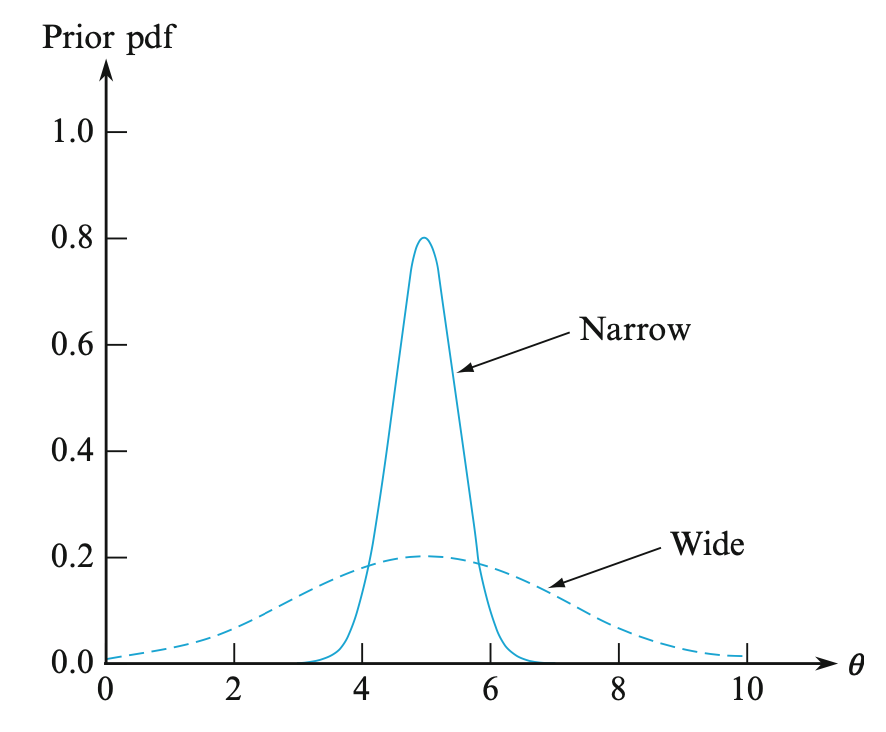
\includegraphics[scale=0.6]{./3_Images/prior_illustration.png}
%    \caption{A narrow concentrated prior about some central value and a wider less informative prior.}
%    \label{fig:prior_illustration}
%    \source{Figure 14.3 in \cite{STK}.}
%\end{figure}


\begin{figure}[H]
    \centering
    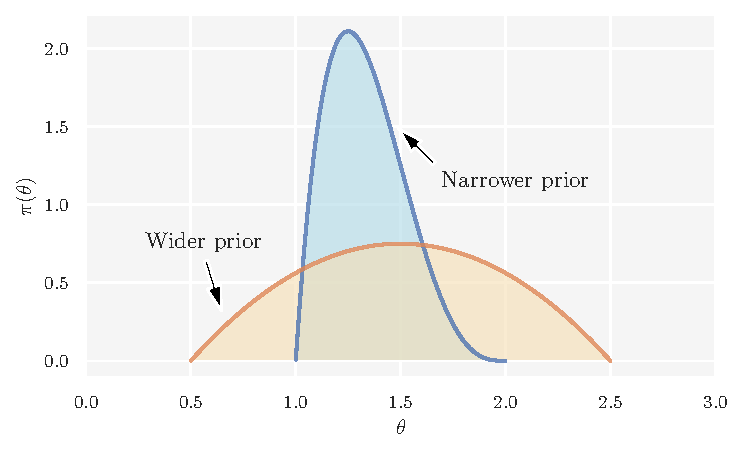
\includegraphics[scale=1.0]{prior_plot}
    \caption{Two prior distributions $\pi (\theta)$. A narrow concentrated prior (more certainty) about some central value and a wider less informative prior (less certainty).}
    \label{fig:prior_illustration}
    %\source{Figure 14.3 in \cite{STK}.}
\end{figure}

Our prior state of knowledge is modified by data $y$, obtained by performing experiments, through the conditional \textit{sampling distribution} $\lhood$. When regarded as a function of $\theta$, for fixed $y$, $\lhood$ is called the \textit{likelihood function}. In order to make probability statements about $\theta$ given sample data $y$, a probabilistic model representing the joint probability distribution for $\theta$ and $y$ must be provided. The joint pmf or pdf can be written as a product of the prior distribution $\prior$ and the likelihood function $\lhood$:

\begin{equation*}
    \joint = \lhood \prior .
\end{equation*}

At this point, Bayes' theorem is used to produce the \textit{posterior distribution}, which represents our state of knowledge about $\theta$ in the light of $y$. A common incarnation of Bayes' theorem is:

\begin{equation}\label{eq:bayes_theorem}
    \posterior = \frac{\joint}{p(y)}  = \frac{\lhood \prior}{p(y)},
\end{equation}

where the marginal probability of the data $p(y) = \int \lhood \prior \dd \theta$ in the case of continuous parameters, or, in the case of a discrete set of parameters, $p(y) = \sum_\theta \lhood \prior$, where the sum is over all possible values of $\theta$.

$p(y)$ is the same for all possible $\theta$, as it does not depend on $\theta$. With fixed $y$, this factor can thus be omitted in parameter inference since it constitutes a normalizing constant and does not enter into determining the relative posterior probabilities of different values of $\theta$. Omitting the factor $p(y)$ yields the unnormalized posterior distribution: 

\begin{equation}\label{eq:bayes_unnorm}
    \posterior \propto p(\theta, y) =  \lhood \prior .
\end{equation}

In this formulation, $\lhood$ is taken as a function of $\theta$ and not $y$.  

The core of Bayesian inference is encapsulated in \autoref{eq:bayes_theorem} and \autoref{eq:bayes_unnorm}. The principal task is to develop the joint probability model $\joint$ and perform the computations to summarize the posterior $\posterior$.


%================================================================
\section{Parameter Inference}\label{sec:param_inference}
%\section{Single-parameter Models}\label{sec:single_inference}
%================================================================  

The way in which Bayes' theorem operates is best seen through examples. In the following we discuss Bayesian inference in the context of statistical models where closed forms are available. Such models are sometimes unrealistic, but their analysis often provides a useful starting point when it comes to constructing more realistic models. The focus of this section will be on how we can summarize the obtained posteriors with various graphical checks and numerical measures. 

%The way in which Bayes’s theorem operates is best seen through examples. In the following we develop some problem formulations to apply Bayesian analysis on for parameter inference. We will focus on situations where closed forms are available, that is, situations where we can use probability models based on the standard distributions. In particular, we will look at probability models based on the binomial and normal distributions. The binomial distribution is motivated from counting exchangeable outcomes, and the normal distribution applies to a random variable that is the sum of many exchangeable or independent terms. Such models are sometimes unrealistic, but their analysis often provides a useful starting point when it comes to constructing more realistic models. The toy problems developed in this section will later serve as benchmark problems. 

%================================================================
\subsection{Single-Parameter Inference}\label{sec:coin_flipping}
%===============================================================

The beta-binomial model is one of the simplest Bayesian models, and useful for introducing important concepts and computational methods in Bayesian analysis. The model is often illustrated in the context of the classical coin-flipping problem, where only a single scalar parameter, the success probability $\theta$, is to be estimated. 

In the coin-flipping problem, we toss a coin $n$ times and record the observations: either \textit{heads} or \textit{tails}. Based on this data, we try to answer questions such as “is the coin fair?”. In order to estimate the fairness of a coin in a Bayesian setting, we need observed data, a probabilistic model of the data generating process, i.e., the likelihood, and priors placed on the unknown model parameters. For this example, we assume that the data-gathering part is already done and we have recorded $y_0$ heads. The fairness of the coin is represented by the $\theta$ parameter, and we say that a coin with $\theta=1$ will always land heads, one with $\theta=0$ always tails and one with $\theta=0.5$ have an equal chance of landing either heads or tails. Assuming that only two outcomes are possible, heads or tails, and the random variable \textit{coin toss} is independent and identically distributed (iid), a candidate for the likelihood is the binomial distribution: 

% p \qty(y \mid \theta)
\begin{equation}\label{eq:coin_flip_likelihood}
    \lhood = \binom{n}{y} \theta^y \qty(1 - \theta)^{n-y}.
\end{equation}

This is a discrete distribution returning the probability of getting $y$ heads (or in general, successes) out of $n$ coin tosses (or in general, trials or experiments) given a fixed value of $\theta$ (probability of success). 

\autoref{fig:binom_distribution} illustrates the binomial distribution for different $\theta$. From the figure we see that $\theta$ indicates how likely it is to obtain a head when tossing a coin, making the binomial distribution a reasonable choice for the likelihood. 

\begin{figure}[H]
    \centering
    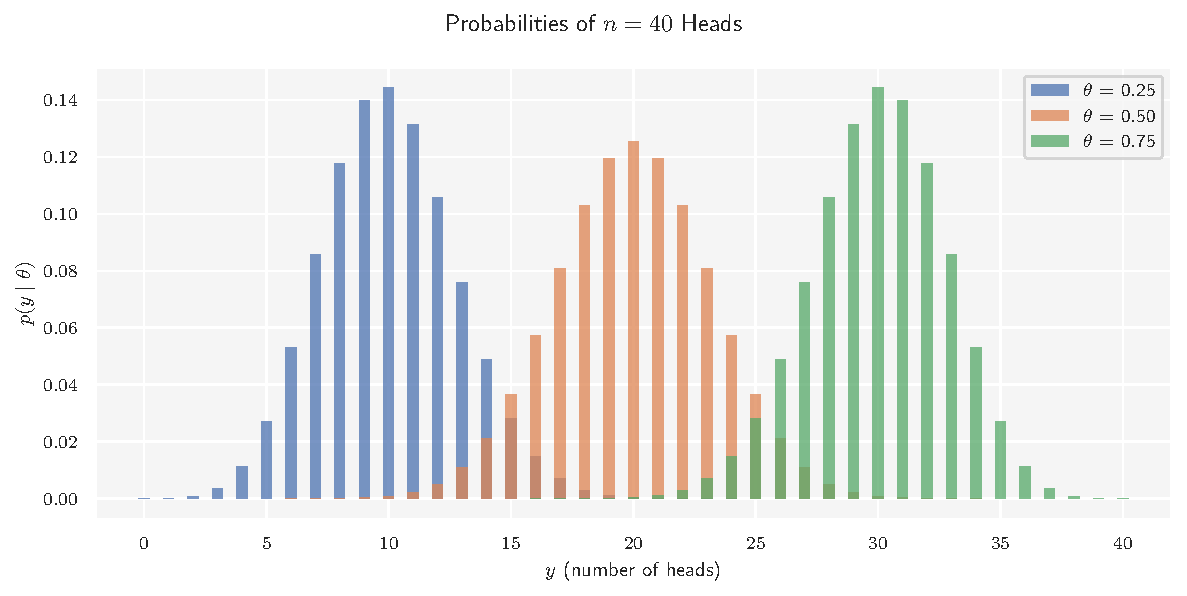
\includegraphics[scale=1]{binomial_distribution}
    \caption{Binomial distributions with $n=40$ coin flips and different success probabilities $\theta$. The coin is biased towards tails when $\theta < 0.5$ and heads when $\theta > 0.5$. For $\theta=0.5$ the coin is unbiased (or fair). The legend indicates the values of the $\theta$.}
    \label{fig:binom_distribution}
    %\source{Figure 14.3 in \cite{STK}.}
\end{figure} 

If the value of $\theta$ is known, the binomial distribution tells us the expected distribution of heads. However, $\theta$ is an unknown model parameter, and thus we need to place a prior on it. For mathematical convenience, we choose a family of prior densities that lead to simple posterior densities. Considered as a function of $\theta$, \autoref{eq:coin_flip_likelihood} is of the form: 
\begin{equation*}
    \lhood \propto \theta^a \qty(1 - \theta)^b.
\end{equation*} 

If the prior density is of the same form, with its own parameterization of $a$ and $b$, then the posterior will also be of this form. Such a prior density can be parameterized as: 

\begin{equation*}
    \prior \propto \theta^{\alpha - 1} \qty(1 - \theta)^{\beta -1},
\end{equation*}

which is the a beta distribution with shape parameters $\alpha>0$ and $\beta>0$. The parameters of the prior distribution are often called \textit{hyperparameters}. In order to ensure that the total probability is 1, the beta function,

\begin{equation*}
    B (\alpha, \beta) = \frac{\Gamma(\alpha)\Gamma(\beta)}{\Gamma(\alpha + \beta)},
\end{equation*}

where $\Gamma (z)$ is the gamma function, can be used as a normalizing constant:

\begin{equation}\label{eq:beta_prior}
    \prior = \frac{1}{B(\alpha, \beta)} \theta^{\alpha -1} (1-\theta)^{\beta -1}.
\end{equation}

The beta distribution is defined on the interval $[0, 1]$. \autoref{fig:beta_distribution} shows the beta distribution with different shape parameters. The figure displays the versatility of the beta distribution; the distribution adopts several shapes, determined by the shape parameters, including the uniform distribution with $\alpha = \beta = 1$. 

\begin{figure}[ht]
    \centering
    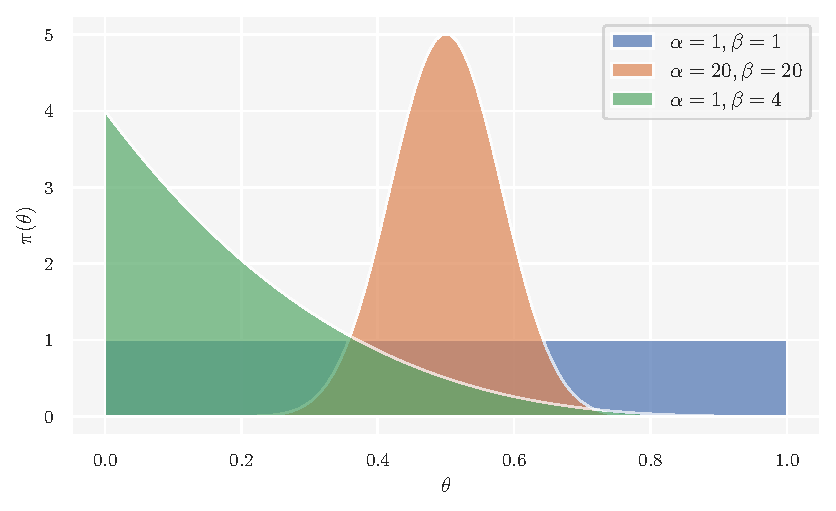
\includegraphics[scale=1]{beta_distribution}
    \caption{The beta prior probability distribution with different parameterizations by the two positive shape parameters. The legend indicates the values of the corresponding shape parameters $\alpha$ and $\beta$. The beta distribution adopts several shapes controlled by the shape parameters; $\alpha=\beta=1$ gives a uniform distribution, $\alpha=\beta=20$ gives a bell curve centered at $\theta=0.5$ and finally $\alpha=1$ and $\beta=2$ gives a reverse J-shaped distribution with a right tail.
    }
    \label{fig:beta_distribution}
    %\source{Figure 14.3 in \cite{STK}.}
\end{figure} 



Bayes' theorem, \autoref{eq:bayes_unnorm}, states that the posterior is proportional to the product of the likelihood and the prior. Thus, for our problem the posterior density for $\theta$ is given as: 

\begin{equation*}
    \pi (\theta \mid y) \propto \binom{n}{y} \theta^y (1-\theta)^{n-y} \frac{1}{B(\alpha, \beta)} \theta^{\alpha-1}(1-\theta)^{\beta -1}.
\end{equation*}

With fixed $n$ and $y$, the factor $\binom{n}{y}$ does not depend on the unknown parameter $\theta$, and neither does the beta function $B(\alpha, \beta)$. Thus can both be treated as constants when calculating the posterior distribution of $\theta$:

\begin{align*}
    \posterior &\propto \theta^y (1-\theta)^{n-y} \theta^{\alpha-1}(1-\theta)^{\beta -1} \\
    &= \theta^{\alpha + y -1} (1-\theta)^{\beta + n-y -1},
\end{align*}

or, more concisely:

\begin{equation}\label{eq:coin_posterior}
    \posterior \propto \theta^{\alpha' -1} (1-\theta)^{\beta' -1},
\end{equation}

with $\alpha'=\alpha+y$ and $\beta' = \beta + n - y$. We recognize that the expression above has the same functional form as the unnormalized beta distribution. The property that the posterior distribution follows the same parametric form as the prior distribution is called \textit{conjugacy}, and we say that the beta prior distribution is a \textit{conjugate prior} for the binomial likelihood.  

fig illustrates how our posterior beliefs are updated in the light of observed data.

\begin{figure}[ht]
    \centering
    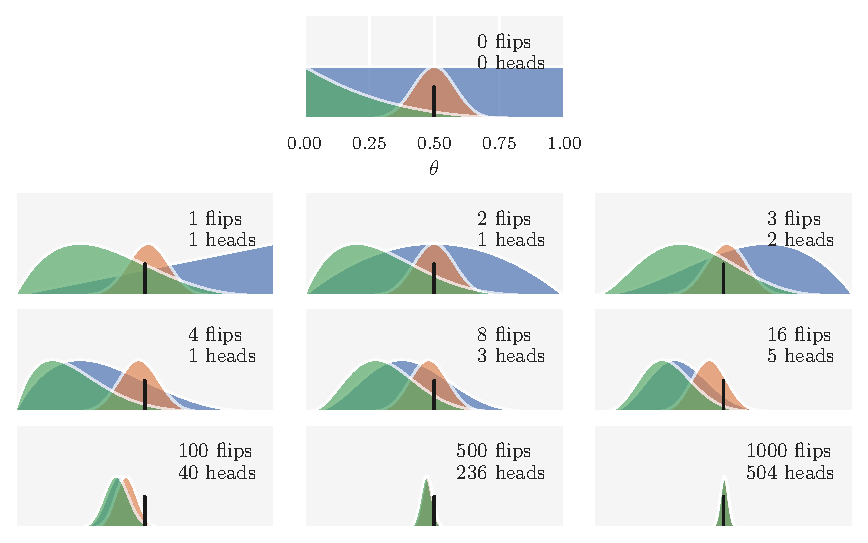
\includegraphics[scale=1]{coin_flip_posterior}
    \caption{The beta prior probability distribution with different parameterizations by the two positive shape parameters. The legend indicates the values of the corresponding shape parameters $\alpha$ and $\beta$. The beta distribution adopts several shapes controlled by the shape parameters; $\alpha=\beta=1$ gives a uniform distribution, $\alpha=\beta=20$ gives a bell curve centered at $\theta=0.5$ and finally $\alpha=1$ and $\beta=2$ gives a reverse J-shaped distribution with a right tail.
    }
    \label{fig:beta_distribution}
    %\source{Figure 14.3 in \cite{STK}.}
\end{figure} 

shows how the posterior pdfs for the different priors evolve, as more and more data become available;


We find that when there are few data, the resulting posteriors are different in detail; as the number of data increases, they all become more sharply peaked and converge to the same answer. This seems quite reasonable. The outcome of only a few flips tells us little about the fairness of the coin. Our state of knowledge after the analysis of these data is, therefore, strongly dependent on what we knew or assumed before the results; hence, the posteriors are somewhat different. As the empirical evidence grows, we are eventually led to the same conclusions irrespective of our initial beliefs; the posterior pdf is then dominated by the likelihood function, and the choice of the prior becomes largely irrelevant.

Two further curious points may be noted: (i) it takes quite a lot of flips to be able to estimate the bias-weighting with some degree of confidence (about a thousand to pin it down between 0.2 and 0.3); (ii) the posterior pdfs for the solid and dotted lines converge together quite quickly, but the dashed case takes much longer. The answer to the first observation is that it just does, but the number of flips required will depend on the actual bias-weighting of the coin. If the coin was tossed ten times and came up tails on every occasion, we would rapidly conclude that it was biased; on the other hand, the result of 45 heads and 55 tails in a hundred flips would still leave us somewhat uncertain as to whether the coin was fair. With regard to the second point, both the flat (solid) and the spiky (dotted) priors encode a large degree of ignorance about the nature of the coin. Despite the peculiar shape of the latter, it is fairly flat for most values of H; the strange-looking spikes at H = 0 and H = 1 disappear as soon as a head and a tail have been observed. The ‘fair-minded’ prior (dashed line), however, claims to be moderately well-informed about the character of the coin regardless of the data. It, therefore, takes much more to be convinced that the coin is not fair. Even though the prior probability for H = 0.5 was about a million times greater than that of H = 0.25, a thousand flips were enough to drag it (kicking and screaming, perhaps) to the conclusion that the value of H was less than 0.3 (but more than 0.2).


FIG text 

Theeffectofdifferentpriors,prob(H|I),ontheposteriorpdfforthebias-weightingof a coin. The solid line is the same as in Fig. 2.1, and is included for ease of comparison. The case for two alternative priors, reflecting slightly different assumptions in the conditioning information I, are shown with dashed and dotted lines.

Theevolutionoftheposteriorpdfforthebias-weightingofacoin,prob(H|{data},I), as the number of data available increases. The figure on the top right-hand corner of each panel shows the number of data analysed; in the early panels, the H or T in the top left-hand corner shows whether the result of that (last) flip was a head or a tail.

%%%




%%%
%%%





%================================================================
\section{Toy Problems for Benchmarking}\label{sec:toy_problems}
%================================================================

Develop problems for benchmarking



Only derive this

%================================================================
\subsection{Gaussian Models}\label{sec:gaussian_models}
%================================================================

normal models important blabla

%================================================================
\subsubsection{With Unknown Mean}
%================================================================

The comprehensive derivation can be found in appendix B. 

Devore, p. 781 

Note that the posterior mean $\mu_0'$ is a weighted average of the prior mean $\mu_0$ and the data mean $\bar{x}$, with weights that are the reciprocals of the prior variance and the variance of $\bar{x}$. It makes sense to define the \textbf{precision} as the reciprocal of the variance because a lower variance implies a more precise measurement and the weights then are the corresponding precisions. Furthermore, the posterior variance is the reciprocal of the sum of the reciprocals of the two variances, but this can be described much more simply by saying that the posterior precision is the sum of the prior precision plus the precision of $\bar{x}$. 

%================================================================
\subsubsection{With Unknown Variance}
%================================================================

The comprehensive derivation can be found in appendix B. 

%================================================================
\subsubsection{With Unknown Mean and Variance}
%================================================================

The comprehensive derivation can be found in appendix B. 




%================================================================
\section{The Influence of the Prior and How to Choose One}\label{sec:prior}
%================================================================

\begin{itemize}
    \item Flat
    \item Uninformative
    \item Diffuse
    \item The Jeffreys’ Prior: Suppose we cannot easily find the natural scale on which the likelihood is in data-translated format, or that such a decomposition does not exist. Jeffreys (1961) proposed a general prior in such cases, based on the Fisher information I of the likelihood. 
    \item When a prior distribution is not integrable it is said to be \textit{improper}
\end{itemize}


%================================================================
\subsection{Conjugate Prior Distributions}
%================================================================

In Bayesian probability theory, if posterior
distributions are in the same family as the prior
distributions, then both prior and posterior are called
conjugate distributions and the prior is called
conjugate prior.

Conjugacy is formally defined as follows. If $\mathcal{F}$ is a class of sampling distributions $p \left(y | \theta \right)$, and $\mathcal{P}$ is a class of prior distributions for $\theta$, then the class $\mathcal{P}$ is \textit{conjugate} for $\mathcal{F}$ if

\begin{equation}
    \pi \left(\theta | y \right) \in \mathcal{P} \, \forall p \left(\cdot | \theta \right) \in \mathcal{F} \land \pi (\cdot) \in \mathcal{P}
\end{equation}

This definition is formally vague since if we choose $\mathcal{P}$ as the class of all distributions, then $\mathcal{P}$ is always conjugate no matter what class of sampling distributions is used. We are most interested in \textit{natural} conjugate prior families, which arise by taking $\mathcal{P}$ to be the set of all densities having the same functional form as the likelihood \cite{ABC_ch1}.

A conjugate prior of a likelihood is a prior that, when used in combination with a given likelihood, returns a posterior with the same functional form as the prior. cite BAP

%================================================================
\section{Prior and Posterior Predictive Checks}
%================================================================

\begin{itemize}
    \item \url{https://docs.pymc.io/notebooks/posterior_predictive.html}
    \item \url{https://avehtari.github.io/masterclass/slides_ppc.pdf}
    \item \url{https://vasishth.github.io/bayescogsci/book/sec-priorpred.html}
    \item \url{https://betanalpha.github.io/assets/case_studies/principled_bayesian_workflow.html#113_Prior_Predictive_Checks}
    \item \url{http://bebi103.caltech.edu.s3-website-us-east-1.amazonaws.com/2018/tutorials/t6a_model_generation_and_prior_predictive_checks.html} python
\end{itemize}

%================================================================
\section{Uncertainty/Sensitivty Analysis in the Bayesian Paradigm}
%================================================================

TODO

\section{Topics} 

In Bayesian inference, posterior beliefs about parameters are updated according to \textit{Bayes' theorem} upon observing data.  

The mean of this posterior distribution gives a point estimate of $\theta$. 

An interval having a posterior probability $.95$ gives a $95\%$ \textit{credibility} interval, an interval within which an unobserved parameter value falls with a particular probability, the Bayesian analogue of a $95\%$ confidence interval \cite[p. 777]{STK}.

Credible intervals 

HDI 

Energy


%================================================================
\subsection{The Prior and Posterior Predictive Distributions}\label{sec:predictive}
%================================================================

BDA, side 7

%================================================================
\section{Summarizing the Posterior}
%================================================================

- mean, median, mode: point estimates

- variance and standard deviation: spread -> uncertainty 

- credible intervals, highest density posterior (hdp) 



%================================================================
\section{Why Bayes?}
%================================================================

End chapter with this? No, move to introduction
